\documentclass{article}

% \usepackage[ansinew]{inputenc} %Bærbar ÆØÅ?

\usepackage{minted}
\usepackage{graphicx} % Allows figures
% \usepackage{tabularx}
\usepackage{amsmath} %math
%Section style
\usepackage{etoolbox} %for configuration of sloppy
\usepackage{xcolor}

\definecolor{secnum}{RGB}{102,102,102}

\makeatletter
    \def\@seccntformat#1{\llap{\color{secnum}\csname the#1\endcsname\hskip 16pt}}
\makeatother
%end section style

{\sloppy}{\hbadness 10000\relax}{}{} %adds hbadness to sloppy
\setlength{\paperheight}{297mm} %Sets the page to an A4
\setlength{\paperwidth}{210mm}        %Sets the page to an A4

\begin{document}

\begin{titlepage}
\begin{center}
\textsc{Introduction to Graphics}\\[0.5cm]
\textsc{Assignment 3: Projections}\\[0.5cm]
\vspace{2 cm}
\begin{tabular}{ll}
Student: & Kasper Passov\\
\end{tabular}
\end{center}
\vspace{5 cm}
\newpage
\end{titlepage}

\section{Problem Description}
Projections is a group of protocala drawing objects 
from a 3d world onto a 2d plane. There are two catagories
of projection, each with its own protocols:
\begin{itemize}
    \item{Parallel projection:} line of sight is a plane parallel to the projection plane.
    \item{Perspective projection:} line of sight originates from a point.
\end{itemize}
This gives perspective projection the interesting feature of gaining a
parllel projection if the distance between the camera and the projection
plane is raised into infinity.\\
The given assignment has us implementing a method of transforming an
arbitrary view volume, into a canonical parallel view volume.
This gives us two types of transformations, one from an arbitrary
parallel view, and one from an arbitrary perspective view.

\section{Implementaion Theory}
\subsection{Parallel projection}
A transformation from a parallel projection into a canonical
parallel view has 4 steps:
\begin{itemize}
    \item{Translate VRP(View reference point) to the origin}
    \item{Rotate the \emph{Eye-Coordinate System}}
    \item{Shear so the DOP(Direction of projection) is parallel to the Z-axis}
    \item{Translate and scale to the \emph{Canonical Orthographic View Volume}}
\end{itemize}
\paragraph{Step 1: Translate VRP to the origin}
Is pretty simply a translation with the negative VRP vector, as the 
VRP vector takes base in origin.
\begin{equation*}
    T(-VRP) =
    \begin{bmatrix}
        1 & 0 & 0 & -vrp_x\\
        0 & 1 & 0 & -vrp_{y}\\
        0 & 0 & 1 & -vrp_{z}\\
        0 & 0 & 0 & 1
    \end{bmatrix}
\end{equation*}
\paragraph{Step 2: Rotate the \emph{Eye-Coordinate System}}
We want our $(u,v,n)$ axis to line up with the $(x,y,z)$ axis,
this is done by the rotation based on VPN. This is done by the 
matrix: 
\begin{equation*}
    R =
    \begin{bmatrix}
        r_{1x} & r_{2x} & r_{3x} & 0\\ 
        r_{1y} & r_{2y} & r_{3y} & 0\\
        r_{1z} & r_{2z} & r_{3z} & 0\\
        0 & 0 & 0 & 1
    \end{bmatrix}
\end{equation*}
where our $R$ vectors are defined as:
\begin{align*}
    R^{T}_{z} &= (r_{1z}, r_{2z}, r_{3z}) = \frac{VPN}{||{VPN}||_2}\\
    R^{T}_{x} &= (r_{1x}, r_{2x}, r_{3x}) = \frac{VUP * R_z}{||VUP * R_z||_2}\\
    R^{T}_{y} &= (r_{1y}, r_{2y}, r_{3y}) = \frac{R_z * R_x}{||R_z * R_x||_2}
\end{align*}
This gives us a projection based in the origin of $(x,y,z)$ coinsiding
with the axises.

\paragraph{Step 3: Shear the DOP}
We now wish to shear the matrix so our DOP is parallel to our z-axis.
The DOP is defined as the length between our View Reference Point
and the Center Window.
\begin{equation*}
    DOP = PRP - CW = (dop_u, dop_v, dop_n, 0)^T
\end{equation*}
To do the transformation we use the following transformed shear matrix:
\begin{equation*}
    Sh_{par} = 
    \begin{bmatrix}
        1 & 0 & -\frac{dop_u}{dop_n} & 0\\ 
        0 & 1 & -\frac{dop_v}{dop_n} & 0\\
        0 & 0 & 1 & 0\\
        0 & 0 & 0 & 1
    \end{bmatrix}
\end{equation*}

This gives us a projection based in the origin and coinsiding
with the axes sof $(x,y,z)$, with a DOP parallel with the z-axis.

\paragraph{Step 4: Translate and scale}
The last part of our parallel projection transformation, is a
translation and scalation into the \emph{Canonical Parallel View Volume}
Moving the front of our view plane onto the XY-plane, and placing CW at the origin.
CW is by definition in the center of our view plane $(u,v)$:
\begin{equation*}
    CW = (cw_u,cw_v,0)^T = (\frac{u_{max} + u_{min}}{2},\frac{v_{max} + v_{min}}{2},0)
\end{equation*}
We translate into our CW
\begin{equation*} 
    T_{par}
    \begin{bmatrix}
        1 & 0 & 0 & \frac{u_{max} + u_{min}}{2}\\ 
        0 & 1 & 0 & \frac{v_{max} + v_{min}}{2}\\
        0 & 0 & 1 & -F\\
        0 & 0 & 0 & 1
    \end{bmatrix}
\end{equation*}
Lastly we scale our view volume into the dimensions
\begin{equation*}
    [-1,1]\cdot[-1,1]\cdot[0,-1]
\end{equation*}
With the matrix
\begin{equation*}
    S_{par}
    \begin{bmatrix}
        \frac{2}{u_{max} + u_{min}} & 0 & 0 & 0\\ 
        0 & \frac{2}{v_{max} + v_{min}} & 0 & 0\\
        0 & 0 & \frac{1}{F - B} & 0\\
        0 & 0 & 0 & 1
    \end{bmatrix}
\end{equation*}


\subsection{Perspective projection}
A transformation from a perspective projection into a canonical
parallel view has 5 steps:
\begin{itemize}
    \item{Translate VRP to the origin}
    \item{Rotate the \emph{Eye-Coordinate System}}
    \item{Translate PRP to the origin}
    \item{Shear so the center line of the \emph{View Volume} is parallel to the Z-axis}
    \item{Scale to the \emph{Canonical Perspective View Volume}}
\end{itemize}
This has some in common with the parallel projection, as step one,
two and 4 are calculatet the same way, so these will be skipped in this
explanation.

\paragraph{Step 3: Translate PRP to origin}
We translate our PRP using the same method as in step 1, but with
$(u,v,n)$ as our perspective is based on that coordinate system.
\begin{equation*}
    T(-PRP) = 
    \begin{bmatrix}
        1 & 0 & 0 & -prp_u\\
        0 & 1 & 0 & -prp_{v}\\
        0 & 0 & 1 & -prp_{n}\\
        0 & 0 & 0 & 1
    \end{bmatrix}
\end{equation*}

\paragraph{Step 4: Shear center line of the \emph{View Volume} to the Z-axis}
We wish to move the center of the View Volume to the Z-axis, this
will be the same transformation as in parallel projection as the 
DOP vector has the same slopes as our perspective center line.

\paragraph{Step 5: Scale to the \emph{Canonical Perspective View Volume}}
The last step involes scaling into the Canonical Perspective View Volume
and is done by the matrix
\begin{equation*}
    S_{par} = 
    \begin{bmatrix}
        \frac{-2prp_n}{(u_{max}-u_{min})(B - prp_n)} & 0 & 0 & 0\\
        0 & \frac{-2prp_n}{(v_{max}-v_{min})(B-prp_n)} & 0 & 0\\
        0 & 0 & \frac{-1}{B-prp_n} & 0\\
        0 & 0 & 0 & 1
    \end{bmatrix}
\end{equation*}


\subsection{Summation}

\paragraph{Parallel}

The above transformation can be summed up as:
\begin{equation*}
    N_{par} = S_{par} \cdot T_{par} \cdot Sh_{par} \cdot R \cdot T(-VRP)
\end{equation*}
Creating a \emph{Canonical Parallel View Volume} from a \emph{World Coordinate System}.

Just for fun we left-multiply this by the following matrix to get the \emph{Orthographic Projection}
\begin{equation*}
    \begin{bmatrix}
        X\\
        Y\\
        0\\
        1
    \end{bmatrix}=
    \begin{bmatrix}
        1 & 0 & 0 & 0\\
        0 & 1 & 0 & 0\\
        0 & 0 & 0 & 0\\
        0 & 0 & 0 & 1
    \end{bmatrix}
    \begin{bmatrix}
        X\\
        Y\\
        Z\\
        1
    \end{bmatrix}
\end{equation*}
and lastly leftmultiply by the \emph{Window-Viewport} matrix:
\begin{equation*}
    M_{WV} = S(\frac{width}{2},\frac{height}{2},1) \cdot T(1,1,0)
\end{equation*}
This last matrix translates and scales our \textbf{Canonical Window}
into a \textbf{Actual Screen View Port}.
Giving us the final transformations:
\begin{equation*}
    M_{par-total} = M_{WV} \cdot S_{par} \cdot T_{par} \cdot Sh_{par} \cdot R \cdot T(-VRP)
\end{equation*}

\paragraph{Perspective}
The above transformations can be summed up as, transforming a 
\emph{World Coordinate System} to a \emph{Canonical Perspective View Volume}:
\begin{equation*}
    N_{par} = S_{per} \cdot Sh_{per} \cdot T_{-PRP} \cdot R \cdot T(-VRP)
\end{equation*}

Just for fun we wish to transform our \emph{Canonical Perspective View Volume}
to the \emph{Canonical Orthographic Projection} using the matrix:
\begin{equation*}
    M_{perpar} =
    \begin{bmatrix}
        1 & 0 & 0 & 0\\
        0 & 1 & 0 & 0\\
        0 & 0 & \frac{1}{1+Z_{max}} & \frac{-Z_{max}}{1+Z_{max}}\\
        0 & 0 & -1 & 0
    \end{bmatrix}
\end{equation*}
and lastly leftmultiply by the \emph{Window-Viewport} matrix:
\begin{equation*}
    M_{WV} = S(\frac{width}{2},\frac{height}{2},1) \cdot T(1,1,0)
\end{equation*}
This last matrix translates and scales our \textbf{Canonical Window}
into a \textbf{Actual Screen View Port}.
Giving us the final transformations for \emph{World-Coordinate} to \emph{Actual Screen View Port}:
\begin{equation*}
    M_{par-total} = M_{WV} \cdot M_{perpar} \cdot S_{per} \cdot Sh_{per} \cdot T(-PRP) \cdot R \cdot T(-VRP)
\end{equation*}
\newpage
\section{Implementaion}
To draw the house i implemented each of the three vertices 
in the GLTriangle doing the following for each, with the exact reason
commented in the code-examples.
\begin{minted}{cpp}
    void GLTriangle::draw() {
        ...
        glBindBuffer(GL_ARRAY_BUFFER, m_BackVBO); // Binds the VBO to the buffer
        glVertexAttribPointer(m_vertexPositionAttribute, 3, 
                              GL_FLOAT, GL_FALSE, 0, 0);
        glDrawArrays(GL_LINE_LOOP, 0, m_numberOfVerticesBack); //draws
        ...
        }

    void GLTriangle::initializeBuffers(ShaderProgram & shaderProgram) {
        ...
        m_numberOfVerticesFront = 5; //number of vectors

        float front[] = { //the positions of all points 
            0.0f, 0.0f, 54.0f,
            16.0f, 0.0f, 54.0f,
            16.0f, 10.0f, 54.0f,
            8.0f, 16.0f, 54.0f,
            0.0f, 10.0f, 54.0f
        };

        glGenBuffers(1, &m_FrontVBO); //generates buffer
        glBindBuffer(GL_ARRAY_BUFFER, m_FrontVBO); //binds the buffer
        glBufferData(GL_ARRAY_BUFFER, sizeof(front), 
                     front, GL_STATIC_DRAW); // binds buffer data
        glVertexAttribPointer(m_vertexPositionAttribute, 3, 
                     GL_FLOAT, GL_FALSE, 0, 0);
        ...
        }
\end{minted}

This with the translation and perspective 
\begin{minted}{cpp}
	modelMatrix = glm::translate(modelMatrix, glm::vec3(0.0f, 0.0f, -100.0f));	
	glm::mat4 perspectiveMatrix = glm::perspective(45.f, 1.f, 2.0f, 120.f);
\end{minted}
draws the following house.\\
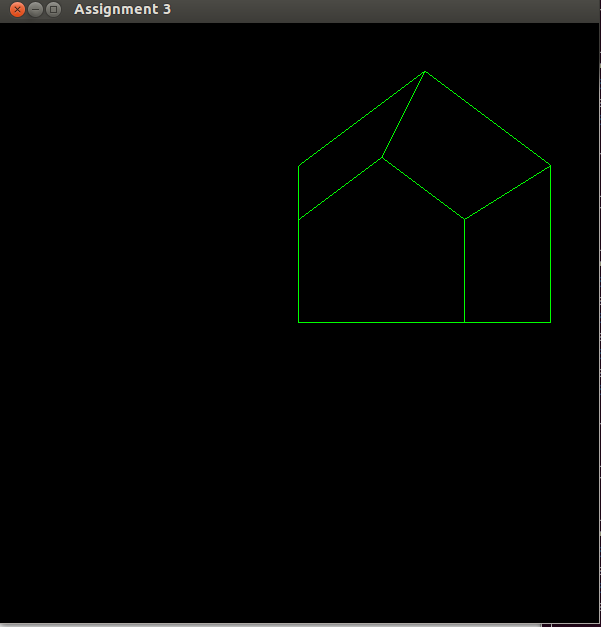
\includegraphics[scale=0.4]{penis1.png}\\
\end{document}

